\documentclass[12pt]{scrartcl}
\usepackage[sexy]{james}
\usepackage[noend]{algpseudocode}
\setlength {\marginparwidth}{2cm}
\usepackage{answers}
\usepackage{array}
\usepackage{tikz}
\newenvironment{allintypewriter}{\ttfamily}{\par}
\usepackage{listings}
\usepackage{xcolor}
\usetikzlibrary{arrows.meta}
\usepackage{color}
\usepackage{mathtools}
\newcommand{\U}{\mathcal{U}}
\newcommand{\E}{\mathbb{E}}
\usetikzlibrary{arrows}
\Newassociation{hint}{hintitem}{all-hints}
\renewcommand{\solutionextension}{out}
\renewenvironment{hintitem}[1]{\item[\bfseries #1.]}{}
\renewcommand{\O}{\mathcal{O}}
\declaretheorem[style=thmbluebox,name={Chinese Remainder Theorem}]{CRT}
\renewcommand{\theCRT}{\Alph{CRT}}
\setlength\parindent{0pt}
\usepackage{sansmath}
\usepackage{pgfplots}

\usetikzlibrary{automata}
\usetikzlibrary{positioning}  %                 ...positioning nodes
\usetikzlibrary{arrows}       %                 ...customizing arrows
\newcommand{\eqdef}{=\vcentcolon}
\newcommand{\tr}{{\rm tr\ }}
\newcommand{\im}{{\rm Im\ }}
\newcommand{\spann}{{\rm span\ }}
\newcommand{\Col}{{\rm Col\ }}
\newcommand{\Row}{{\rm Row\ }}
\newcommand{\dint}{\displaystyle\int}
\newcommand{\dt}{\ {\rm d }t}
\newcommand{\PP}{\mathbb{P}}
\newcommand{\horizontal}{\par\noindent\rule{\textwidth}{0.4pt}}
\usepackage[top=3cm,left=3cm,right=3cm,bottom=3cm]{geometry}
\newcommand{\mref}[3][red]{\hypersetup{linkcolor=#1}\cref{#2}{#3}\hypersetup{linkcolor=blue}}%<<<changed

\tikzset{node distance=4.5cm, % Minimum distance between two nodes. Change if necessary.
         every state/.style={ % Sets the properties for each state
           semithick,
           fill=cyan!40},
         initial text={},     % No label on start arrow
         double distance=4pt, % Adjust appearance of accept states
         every edge/.style={  % Sets the properties for each transition
         draw,
           ->,>=stealth',     % Makes edges directed with bold arrowheads
           auto,
           semithick}}


% Start of document.
\newcommand{\sep}{\hspace*{.5em}}

\pgfplotsset{compat=1.18}
\begin{document}
\title{AMSC460: Homework 1}
\author{James Zhang\thanks{Email: \mailto{jzhang72@terpmail.umd.edu}}}
\date{\today}

\definecolor{dkgreen}{rgb}{0,0.6,0}
\definecolor{gray}{rgb}{0.5,0.5,0.5}
\definecolor{mauve}{rgb}{0.58,0,0.82}

\lstset{frame=tb,
  language=Java,
  aboveskip=3mm,
  belowskip=3mm,
  showstringspaces=false,
  columns=flexible,
  basicstyle={\small\ttfamily},
  numbers=left,
  numberstyle=\tiny\color{gray},
  keywordstyle=\color{blue},
  commentstyle=\color{dkgreen},
  stringstyle=\color{mauve},
  breaklines=true,
  breakatwhitespace=true,
  tabsize=3
}

\maketitle

$0.$ \textbf{Review Questions}

\begin{enumerate}[(a)]
  \item Scientific computing aims to use computers to use discrete or piecewise solutions to empirically approximate 
  a continuous problem. Algorithms are employed to solve these problems efficiently, accurately, and reliably. 
  on the other hand, the idea behind these algorithms is numerical analysis. 
  \item If $|u|$ is large, then relative error is used and if $|u|$ is very small, 
  then relative error is not a good measurement. For example, if $u = 1000$ and $v = 1001$, then 
  relative error is better because relative error is $0.001$ whereas the absolute error is $1$ and looks worse, when in reality, 
  this model is quite accurate. On the other hand, if $u = 0.00001$ and $v = 0.00003$, then 
  the relative error is $2$ which looks huge, but in reality, the model made a good prediction because 
  the absolute error is only $0.00002$.
  \item A major difference between the nature of discretization error and roundoff error is that 
  \textit{any} computation with a real number involves roundoff error. Furthermore, unlike 
  roundoff errors, discretization errors have a smooth structure which can be exploited. In practice, in successful
  model approximations, discreitzation errors dominate roundoff errors in terms of magnitude.
  \item Roundoff errors are inevitable due to the way all computers store floating point numbers. 
  If the accumulated roundoff error is smaller than the problem's required level of precision, then the 
  predicted model output is okay; otherwise the algorithm needs to be redefined and re-executed such that 
  the rounding errors do not compound throughout calculations. Usually, linear accumulation of errors is unpreventable, 
  whereas exponential error accumulation cannot be tolerated. 
  \item Accuracy is how close the model output is to the ground truth. Efficiency describes how long the algorithm 
  and computation take to run. Efficiency is affected by the researcher's choices of computer language, algorithmic implementation, 
  underlying hardware, and it can be affected by theoretical properties such as the rate of convergence of the algorithm. Robustness is 
  if the solution algorithm works under various conditions. For example, returning the correct answer within 
  tolerable error bounds, or returning the correct error in unsuitable conditions. 
  \item Note that any given polynomial can be rewritten as 
  \[P(x) = ((((a_n x + a_{n-1})x) + a_{n-2})x + \cdots + a_1)x + a_0\]
  Each degree requires one addition and one multiplication, and so therefore there are $n + n = 2n$
  operations, which is $\mathcal{O}(n)$ time complexity.
  \item Problem conditioning describes when a small change in the data produces a drastic change in the solution algorithm's output, whereas 
  algorithm stability describes the solution's robustness to small pertubations and errors that occur during the data. 
  
\end{enumerate}

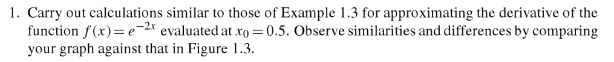
\includegraphics[width=15cm]{1.png}

\begin{proof}[Solution]
  Using a Taylor Series to approximate this model yields 
  \[f(x_0 + h) = f(x_0) + hf'(x_0) + \frac{h^2}{2}f''(x_0) + \cdots\]
  Solving for $f'(x_0)$, we get 
  \[f'(x_0) = \frac{f(x_0 + h) - f(x_0) - \frac{h^2}{2}f''(x_0)}{h} = \frac{f(x_0 + h) - f(x_0)}{h} - \frac{h}{2}f''(x_0)\]
  Below is the code and the graph showing the combined effect of discretization and roundoff errors, and a dashed line 
  showing the discretization error without roundoff error.

\begin{lstlisting}[language=Matlab]
  x0 = 0.5;
  e = exp(1);
  f0 = e^(-2 * x0);
  fp = -2 * f0;
  i = -20:0.5:0;
  h = 10.^i;
  err = abs(fp - (e.^(-2 * (x0 + h)) - f0)./h);
  d_err = 2.*h * e^(-2 * x0);
  loglog(h, err, '-*');
  hold on;
  loglog(h, d_err, 'r-.');
  xlabel('h')
  ylabel('Absolute Error')
\end{lstlisting}
\begin{center}
  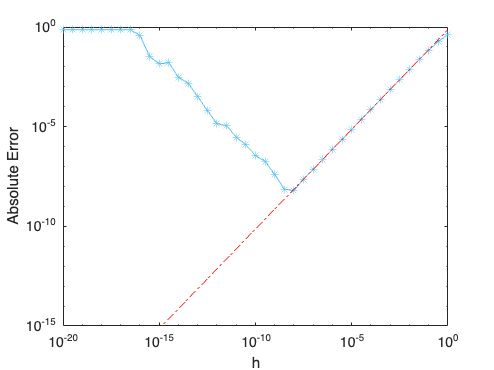
\includegraphics[width=7cm]{g1.png}
\end{center}  

This graph illustrates a lot of similarities to Figure 1.3 in the book. For example, 
the absolute error is relatively constant slightly under $10^0 = 1$ in both graphs. 
At $x = 10^{-14}$. both errors start decreasing almost linearly. However, at around 
$x = 10^{-8}$, the errors start increasing linearly and follow the red-dashed line, 
which means that the absolute error gets ver similar to the discretization error without roundoff error.

\end{proof}

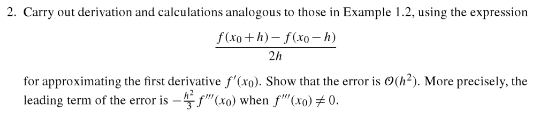
\includegraphics[width=15cm]{2.png}

\begin{proof}[Solution]

  Note that using Taylor Series approximation, we immediately get both of the following 
  \begin{align}
    f(x_0 + h) = f(x_0) + hf'(x_0) + \frac{h^2}{2}f''(x_0) + \frac{h^3}{3!}f'''(x_0) + \cdots\\
    f(x_0 - h) = f(x_0) - hf'(x_0) + \frac{h^2}{2}f''(x_0) - \frac{h^3}{3!}f'''(x_0) + \cdots
  \end{align}
  where for the $f(x_0 - h)$ expansion, the terms with $h$ raised to an odd power are substracted.
  Now, when we subtract $(2)$ from $(1)$, observe that 
  \[f(x_0 + h) - f(x_0 - h) = 2hf'(x_0) + \frac{2h^3}{3!}f'''(x_0) + \frac{2h^5}{5!}f^{(5)}(x_0) + \cdots\]
  Dividing every term by $2h$, we get
  \begin{align}
    f'(x_0) = \frac{f(x_0 + h) - f(x_0 - h)}{2h} - \frac{h^2}{3!}f'''(x_0) - \frac{h^4}{5!}f^{(5)}(x_0) + \cdots
  \end{align}
  Thus, the error is 
  \begin{align}
    \text{Error} = f'(x_0) - \frac{f(x_0 + h) - f(x_0 - h)}{2h} = -\frac{h^2}{3!}f'''(x_0) - \cdots
  \end{align}

  To show that the error is $\mathcal{O}(h^2)$, let $C = 100$ and let $q = 2$. As $h$ decreases, 
  the $h^2$ term will be the largest contributing term, and for all $h$ small enough, we will have the following
  \[|e| \leq 100h^2\]
  \[\frac{h^2}{3!}f'''(x_0) + \frac{h^4}{5!}f^{(5)}(x_0) + \cdots + \frac{h^{2i}}{(2i + 1)!}f^{(2i + 1)}(x_0)\leq 100h^2, \text{ for } i \in \NN\]

  It's clear that when $f'''(x_0) \neq 0$, the leading term of the error is nonzero and it is $-\frac{h^2}{3!}f'''(x_0)$.

  \begin{lstlisting}[language=Matlab]
    x0 = 1.2;
    f0 = sin(x0);
    fp = cos(x0);
    h = [1e-1, 1e-2, 1e-3, 1e-4, 1e-7, 1e-8, 1e-9, 1e-10, 1e-11, 1e-13, 1e-15, 1e-16];
    err = abs(fp - (sin(x0 + h) - sin(x0)) ./ h);
    loglog(h, err, '-*');
    hold on;
    xlabel('h')
    ylabel('Absolute Error')
    % Create a table
    T = table(h', err', 'VariableNames', {'h', 'AbsoluteError'});
    % Display the table
    disp(T);
  \end{lstlisting}

  \begin{center}
    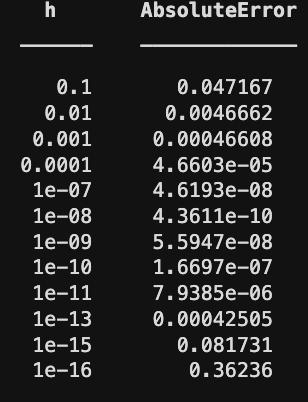
\includegraphics[width=6cm]{table.png}
  \end{center}
\end{proof}

\end{document}

